\documentclass[modern]{aastex631}
%\documentclass[twocolumn]{aastex631}

\usepackage{amsmath}
\usepackage{soul}

% Abundance and stellar macros
\newcommand{\mgfe}[0]{[{\rm Mg/Fe}]} 
\newcommand{\Acc}{A_{\rm cc}}
\newcommand{\AIa}{A_{\rm Ia}} 
\newcommand{\RIa}{R_{\rm Ia}^X}
\newcommand{\aIa}{\alpha_{\rm Ia}}
\newcommand{\acc}{\alpha_{\rm cc}}
\newcommand{\afe}[0]{[\alpha/{\rm Fe}]}
\newcommand{\femg}{[{\rm Fe}/{\rm Mg}]} 
\newcommand{\xmg}{[{\rm X}/{\rm Mg}]} 
\newcommand{\mgh}{[{\rm Mg}/{\rm H}]}
\newcommand{\feh}[0]{[{\rm Fe/H}]} 
\newcommand{\pIa}{p_{\rm Ia}^{\rm X}}
\newcommand{\pcc}{p_{\rm cc}^{\rm X}}
\newcommand{\fcc}{f_{\rm cc}}
\newcommand{\xfe}{[{\rm X}/{\rm Fe}]} 
\newcommand{\pIasun}{p_{\rm Ia, \odot}^{\rm X}}
\newcommand{\pccsun}{p_{\rm cc, \odot}^{\rm X}}
\newcommand{\logg}{\log(g)}
\newcommand{\teff}{T_{\rm eff}}
\newcommand{\kpc}{\rm \; kpc}
\newcommand{\kel}{\rm \; K}
\newcommand{\msun}{M_{\odot}}
\newcommand{\rgc}{R_{\rm GC}}
\newcommand{\msunvice}{M_{\odot}/M_{\odot \rm formed}}
\newcommand{\MZAMS}{M_{\rm ZAMS}}
\newcommand{\Msun}{M_{\odot}}
\newcommand{\qIax}{q_{\rm Ia}^{\rm X}}
\newcommand{\qccx}{q_{\rm cc}^{\rm X}}
\newcommand{\qagbx}{q_{\rm AGB}^{\rm X}}
\newcommand{\qIa}{q_{\rm Ia}}
\newcommand{\qcc}{q_{\rm cc}}
\newcommand{\qagb}{q_{\rm AGB}}
\newcommand{\Aagb}{A_{\rm AGB}}
\newcommand{\eumg}{[{\rm Eu}/{\rm Mg}]} 
\newcommand{\mgmn}{[{\rm Mg}/{\rm Mn}]} 
\newcommand{\alfe}{[{\rm Al}/{\rm Fe}]} 
\newcommand{\omg}{[{\rm O}/{\rm Mg}]} 
\newcommand{\xo}{[{\rm X}/{\rm O}]} 
\newcommand{\xh}{[{\rm X}/{\rm H}]} 
\newcommand{\angstrom}{\textup{\AA}}
\newcommand{\ejg}[1]{\textcolor{red}{EJG: #1}}

%% Reintroduced the \received and \accepted commands from AASTeX v5.2
%\received{March 1, 2021}
%\revised{April 1, 2021}
%\accepted{\today}

%\submitjournal{ApJ}

\newcommand{\name}{\textsl{Foo}} % Hogg's just making this up; change it!!
\newcommand{\documentname}{\textsl{Article}}

\shorttitle{data-driven few-process model for nucleosynthesis}
\shortauthors{griffith and hogg}
\addtolength{\topmargin}{-0.4in} % trust in Hogg
\addtolength{\textheight}{0.7in} % trust in Hogg
\setlength{\parindent}{1.6em}
\renewcommand{\paragraph}[1]{\bigskip\par\noindent{\textbf{#1}}~---}
\sloppy\sloppypar\raggedbottom\frenchspacing % Trust Hogg

\graphicspath{{./}{Figures/}}
\begin{document}

\title{\name: A data-driven few-process model for nucleosynthesis}

\correspondingauthor{Emily J. Griffith}
\email{Emily.Griffith-1@colorado.edu}

\author[0000-0001-9345-9977]{Emily J. Griffith}
\altaffiliation{NSF Astronomy and Astrophysics Postdoctoral Fellow}
\affiliation{Center for Astrophysics and Space Astronomy, Department of Astrophysical and Planetary Sciences, University of Colorado, 389~UCB, Boulder,~CO 80309-0389, USA}

\author[0000-0003-2866-9403]{David W. Hogg}
\affiliation{Center for Cosmology and Particle Physics, Department of Physics, New York University, 726~Broadway, New~York,~NY 10003, USA}
\affiliation{Max-Planck-Institut f{\"u}r Astronomie, K{\"o}nigstuhl 17, D-69117 Heidelberg, Germany}
\affiliation{Flatiron Institute, 162 Fifth Avenue, New~York,~NY 10010, USA}

% \author[0000-0001-7775-7261]{David H. Weinberg}
% \affiliation{The Department of Astronomy and Center of Cosmology and AstroParticle Physics, The Ohio State University, Columbus, OH 43210, USA}
% \affiliation{The Institute for Advanced Study, Princeton, NJ, 08540, USA}

\begin{abstract}\noindent % trust Hogg
Stellar surface abundances look like they are produced by two dominant processes, one prompt and one delayed.
We analyze YYY abundance ratios (ratioed to Mg) for XXXX stars from APOGEE DR17 with a flexible two-process model, in which all element process amplitudes are free parameters.
The two-process model describes each element abundance of each star as the vector sum of a CCSN and SNIa process.
Prior work derives process amplitudes from median observed high-Ia and low-Ia abundance trends; we relax these assumptions and simultaneously fit all model parameters to the data, with only minimal constraints to keep the processes interpretable.
We compare fit parameters from this new method to those derived from prior work [that the two methods produce similar results but with XXX differences and identify similar outlier stars??].
Our flexible method---dubbed \name---tests the validity of the standard two-process assumptions, such as Mg being a pure CCSN element, and that Solar abundances are generated by a roughly half-half combination of CCSN and SNIa processes.
We find [that the assumptions of prior work are generally confirmed. But that the inferred Fcc value of Fe peak elements is strongly dependent upon the chosen CCSN process strength for Fe].
We capitalize on the flexibility to explore the addition of a third process, agnostic about its origin.
The third process most improves [X elements? most significant for X elements?].
Most importantly, \name{} can be extended to populations at very low metallicity, and populations without two clear abundance sequences, such as the LMC/SMC, Sagittarius, and Gaia-Enceladus (??), making it a general diagnostic for enrichment; in principle, it can also be used to constrain fundamental nucleosynthetic parameters.
\end{abstract}

\keywords{foo --- bar}

\section*{}\clearpage
HOGG SAY: Here are some things to do or think about:
\begin{itemize}
  \item Should we think of this as a 2-process model or as a $K$-process model, where $K$ is often 2? I'm leaning towards $K$.
  \item \ejg{I like the K-process model. (This is named $N$-Process model in W22)}
  \item What are we going to do in terms of interpreting the results? These process vectors aren't exactly yields; they are something way more complicated, right?
  \item \ejg{Interpret in terms of $\fcc$. Can also make inferences about the metalicity dependence of SNIa/CCSN enrichment to given elements based on how $\qcc$ and $\qIa$ evolve with time.}
\end{itemize}

\section{Introduction}\label{sec:intro}

After hydrogen, helium, lithium, and beryllium, essentially all other naturally occurring elements are made in stars, and the collisions of stars.
%We are literally made of star stuff.
Stellar surface abundances---the abundances measured by taking a spectrum of a stellar photosphere---are thought to deliver a relatively unprocessed (for most elements) record of the element abundances in the gas from which the star formed (though see \ejg{Add citations}).
These birth abundances were set by a combination of nucleosynthetic processes involved in making heavy atomic nuclei, and astrophysical processes involved in delivering atoms from stellar interiors to star-formation sites \citep[e.g.,][]{johnsonja2020}.
Thus nuclear physics and a wide swath of astrophysics are critically intertwined in our understanding of stellar surface abundances, motivating theoretical, experimental, and observational work.

At the present day, stellar surface abundances are not very well explained by \textsl{ab initio}, physics-driven models.
Yields vary from set to set, as they are dependent on progenitor properties and explosion assumptions \citep[e.g.,][]{rybizki2017, griffith2021b}. 
The wide parameter space of progenitor and supernovae models coupled with uncertainties in reaction rates and explosion physics hinder the creation of an accurate nucleosynthetic model from theory alone.
In the long run, it is incumbent upon us to understand these issues and correct the assumptions or calculations underlying our nucleosynthetic and astrophysical models.
In the short run, however, we gather data---tens of millions of abundance measurements on millions of stars in different astronomical surveys such as RAVE, SEGUE, LAMOST, Gaia-ESO, APOGEE/MWM, GALAH, and H3 \citep{steinmetz2006, yanny2009, gilmore2012, desilva2015, luo2015, majewski2017, conroy2019}.
This raises the question: \emph{Can we take a data-driven approach to nucleosynthesis?}

In this \documentname{}, we build a purely data-driven model for the surface element abundances observed in stars.
We treat each star as being a linear combination of nucleosynthetic processes, beginning with one that is primarily responsible for the $\alpha$-element Mg \citep[core collapse supernovae (CCSN), e.g.][]{andrews2017}, and one that is primarily \emph{not} (Type-Ia supernovae (SNIa)).
Beyond that up-front assumption, we try to be agnostic about how the elements are produced.

We build upon the work of \citet[][hereafter G22]{griffith2019, griffith2022} and \citet[][hereafter W22]{weinberg2019, weinberg2022}, who used the bimodality in [Mg/Fe] vs. [Fe/H] \citep[e.g.,][]{fuhrmann1998, bensby2003, adibekyan2012} to separate stars into populations with high and low SNIa enrichment. Using the median [X/Mg] vs. [Mg/H] abundance trends, these works explain data from the \textsl{GALAH}\footnote{GALAH = GALactic Archaeology with HERMES.} and SDSS-IV \textsl{APOGEE}\footnote{APOGEE = Apache Point Observatory Galactic Evolution Experiment, part of the Sloan Digital Sky Survey} surveys, respectively, with a two-process model. Because the median abundance trends in [X/Mg] vs. [Mg/H] space are largely insensitive to aspects of chemical evolution, such as outflows and variations in star formation history \citep{weinberg2019}, the population abundance trends are set by the nucleosynthetic processes and can be used to empirically constrain Galactic enrichment. To fit the two-process model to survey data, G22 and W22 assume that Mg is purely produced by CCSN, Fe is produced in equal amounts by CCSN and SNIa, and that the CCSN/SNIa yields of Mg and Fe are metallicity independent. While the first assumption is firmly grounded in nucleosynthetic theory \citep[e.g.,][]{andrews2017, rybizki2017}, the others are based on APOGEE abundance patterns and may not be realistic constraints.

Beyond the two-process model, many elements have contributions from additional nucleosynthetic processes, such as the rapid ($r$) and slow ($s$) neutron capture processes \citep{arlandini1999, bisterzo2014} in asymptotic giant branch (AGB) stars \citep[e.g.,][]{simmerer2004, karakas2016} and merging neutron stars \citep{kilpatrick2017}, or atypical supernovae explosion. After predicting stellar abundances from $\feh$ and $\mgfe$, \citet{ting2022} identify correlated abundance residuals that are unexplained by observational uncertainties, indicative of additional nucleosynthetic processes that standard disk CCSN and SNIa enrichment cannot explain. Results from G22 and W22 support this conclusion, and both works attempt to add additional processes to their models to account for non-CCSN and non-SNIa enrichment, though in a very restrictive manner.

To date, survey abundances have not been fully exploited to create a data-driven model of nucleosynthesis. While works such as \citet{ting2012}, \citet{casey2019}, and \citet{ratcliffe2022} effectively use clustering algorithms to identify elements with like sources and reduce abundance dimensionality, the results are difficult to translate into a model of nucleosynthesis. Clustering components can be linked to nucleosynthesis sources and enrichment history, but cannot be used to describe the enrichment of a single star.
\ejg{Add more description of these works?}

In this work, our main innovations are to relax the assumptions made in G22 and W22, to be more agnostic about the nucleosynthetic processes, and to be more principled with the measurements or inferences from data. In our model, we find the intersection between reliable facts about nucleosynthesis and good abundance measurements to build an edifice of nucleosynthesis.  \ejg{Add more about high-quality metallicity labels and our model.} 

This paper is organized as follows. In Section~\ref{sec:data} we describe the APOGEE data and the stellar samples employed in this paper. In Section~\ref{sec:model} we outline our $K$-process model, the assumptions we make, and the implementations of constraints and regularization. We apply the data-driven $K$-process model to the APOGEE data in Section~\ref{sec:optimize} and compare our results to those of W22 in Section~\ref{sec:results_W22}. In Section~\ref{sec:results_broad} we extend the optimization to a broader data sample, discussing the behavior at low metallicity and displaying the power of our optimized K-process abundances labels. Finally, we summarize our results in Section~\ref{sec:summary}


%The benefit we will gain from this is better performance at fitting the data.
%The cost we might pay is a possible reduction in interpretability.
%We'll come back to all that at the end.

%\ejg{Placeholder. We attempt to find the intersection between reliable facts about nucleosynthesis and good abundance measurements. We are trying to build an edifice of nucleosynthesis on a small number of facts. Because Mg is well-measured and well-understood theoretically, it's a good foundation for our model. We have a degeneracy with Fe because we don't have a nucleosynthesis fact.}




\section{Data Samples}\label{sec:data}

In this paper, we employ stellar abundances from APOGEE DR17 \citep{abdurrouf2022}, part of SDSS-IV \citep{majewski2017}. The APOGEE survey obtains high-resolution ($R\sim22,500$) near-infrared (IR) observations \citep{wilson2019} for stars in the Galactic disk, halo, bulge, and nearby satellites/streams. Observations are taken with two nearly identical spectrographs on the 2.5m Sloan Foundation telescope \citep{wilson2019} at Apache Point Observatory in New Mexico and the 2.5m du Pont Telescope \citep{bowen1973} at the Las Companas Observatory in Chile. Spectral data are reduced and calibrated with the APOGEE data processing pipeline \citep{nidever2015}, after which stellar parameters and abundances are calculated with ASPCAP \citep[APOGEE Stellar Parameter and Chemical Abundance Pipeline][]{holtzman2015, garcia2016}. See \citet[][DR16]{jonsson2020} and Holtzman et al. (in prep., DR17) for a more detailed description of APOGEE data reduction and analysis, and \citet{zasowski2013, zasowski2017} and \citet{santana2021} for a discussion of survey targeting.

APOGEE DR17 reports stellar parameters, including $\teff$ and $\logg$, as well as 20 elemental abundances: C, \ion{C}{1}, N, O, Na, Mg, Al, Si, S, K, Ca, \ion{Ti}{1}, \ion{Ti}{2}, V, Cr, Mn, Fe, Co, Ni, and Ce for 657,135 stars. Among these elements and ions, some are measured more precisely than others. We exclude Ti from our analysis as there are large differences between the abundances derived from the \ion{Ti}{1} and \ion{Ti}{2} lines \citep{jonsson2020}. We also exclude P, as the P abundances are measured from a few very weak spectra features, and the abundance distribution displays strong artifacts \citep{jonsson2020}. Among the remaining elements, we note the following concerns: weak Na spectral features, large abundances scatter in S, significant systematic artifacts in Cr abundances at super-solar metallicities, strong unaccounted for NLTE effects on Mn abundances, and large abundance scatter in Co and Ce--both derived from one line. Further, we note that DR17 is the first time Ce abundances have been included in APOGEE data products. For a more detailed discussion of abundance systematics and their effects on population trends, see \citet{jonsson2020} and \citet{griffith2021a}.

% \begin{itemize}
% \itemsep0em
%     \item Na - Spectral features are weak, one of the least precise elements in APOGEE (but matches optical data pretty well)
%     \item S - Large abundance scatter in observations and no verification with optical data
%     \item Cr - Significant systematic artifacts at super solar metallicity \citep{griffith2021a}
%     \item Mn - Strong NLTE effects exist that are not taken into account
%     \item Co - Abundance derived from one line, causing larger abundance scatter
%     \item Ce - Abundance derived from one line. DR17 is the first time Ce abundances have been included in APOGEE data products. 
%     \item Al,  V, and Mn require large offsets to place solar metallicity stars at solar [X/Fe].
% \end{itemize}

In this paper, we will explore two subsamples of APOGEE DR17 data: (1) the W22 sample, optimized to minimize statistical and systematic errors while probing a large portion of the Galactic disk, and (2) a sample with less stringent cuts, but better coverage of the low-metallicity ([Fe/H] $< -0.5$) disk. We discuss the model fits to the W22 sample in Section~\ref{sec:optimize} and ~\ref{sec:results_W22} and the fits the expanded sample in Section~\ref{sec:results_broad}.

\subsection{W22 Sample}

W22 select a subset of APOGEE DR17 stars with the goal of minimizing statistical errors from poor observations and systematic errors from abundance trends with $\teff$ and/or $\logg$ while preserving a sufficient number of stars to conduct a meaningful statistical analysis across the Galactic disk. To remove poor quality data points, W22 require ASPCAP flags \texttt{STAR\_BAD} \texttt{NO\_ASPCAP\_RESULT} equal zero and remove all stars with \texttt{FE\_H\_FLAG} or \texttt{MG\_FE\_FLAG} set. They only include stars from the main survey sample (\texttt{EXTRATARG} = 0), and use named abundances (\texttt{X\_FE}), as recommended by \citet{jonsson2020}. In addition to these quality cuts, W22 apply the following sample selection:
\begin{itemize}
\itemsep0em
    \item $R=3-13$ kpc, $|Z| \leq 2$ kpc (distances from \citealp{leung2019})
    \item $-0.75 \leq \mgh \leq 0.45$
    \item S/N $\geq 200$ for $\mgh > -0.5$ and S/N $\geq 100$ for $\mgh < -0.5$
    \item $\logg = 1-2.5$ dex
    \item $\teff = 4000-4600$ K
\end{itemize}
By selecting stars from a small range of $\logg$ and $\teff$, W22 eliminate the red clump stars \citep{vincenzo2021a} and minimize stellar parameter-dependent abundance trends \citep[see][]{griffith2021a}. The cuts result in a sample of 34,410 stars. 

W22 present abundance for Mg, O, Si, S, Ca, C+N, Na, Al, K, Cr, Fe, Ni, V, Mn, Co, and Ce. In the analysis of each element, X, W22 drop stars with \texttt{X\_FE\_FLAG} (maximum of $\sim 560$ for Ce). While the surface abundances of C and N differ from the stellar birth abundances for RGB stars due to the CNO processes and dredge up events \citep{iben1965, shetrone2019}, the total C+N abundance remains constant. W22 consider C+N as an element in their analysis, taking [(C+N)/H] to be 
\begin{equation}
    [\text{C+N}/\text{H}] = \log_{10}(10^{\text{[C/H]}+8.39} + 10^{\text{[N/H]}+7.78}) - \log_{10}(10^{8.39} + 10^{7.78})
\end{equation}
using logarithmic solar abundances for C (8.39) and N (7.78) from \citet{grevesse2007}.

%\ejg{W22 use X/Fe error from APOGEE and don't convert it to X/Mg....Use C/Fe error for the C+N value because the ratio is mostly C... Need error discussion here and in next section.}

In this paper, we will analyze the same set of stars and elements as W22 (denoted ``W22 sample''), adopting the same definition of [C+N/H]. We plot the distribution of abundances in [X/Mg] vs. [Mg/H] for this sample in Figure~\ref{fig:w22_xmg}. All elemental abundances have zero-point offsets applied and have been de-trended for correlations with $\teff$, as in W22 (see their Table 1). 

\begin{figure*}[htb!]
    \centering
    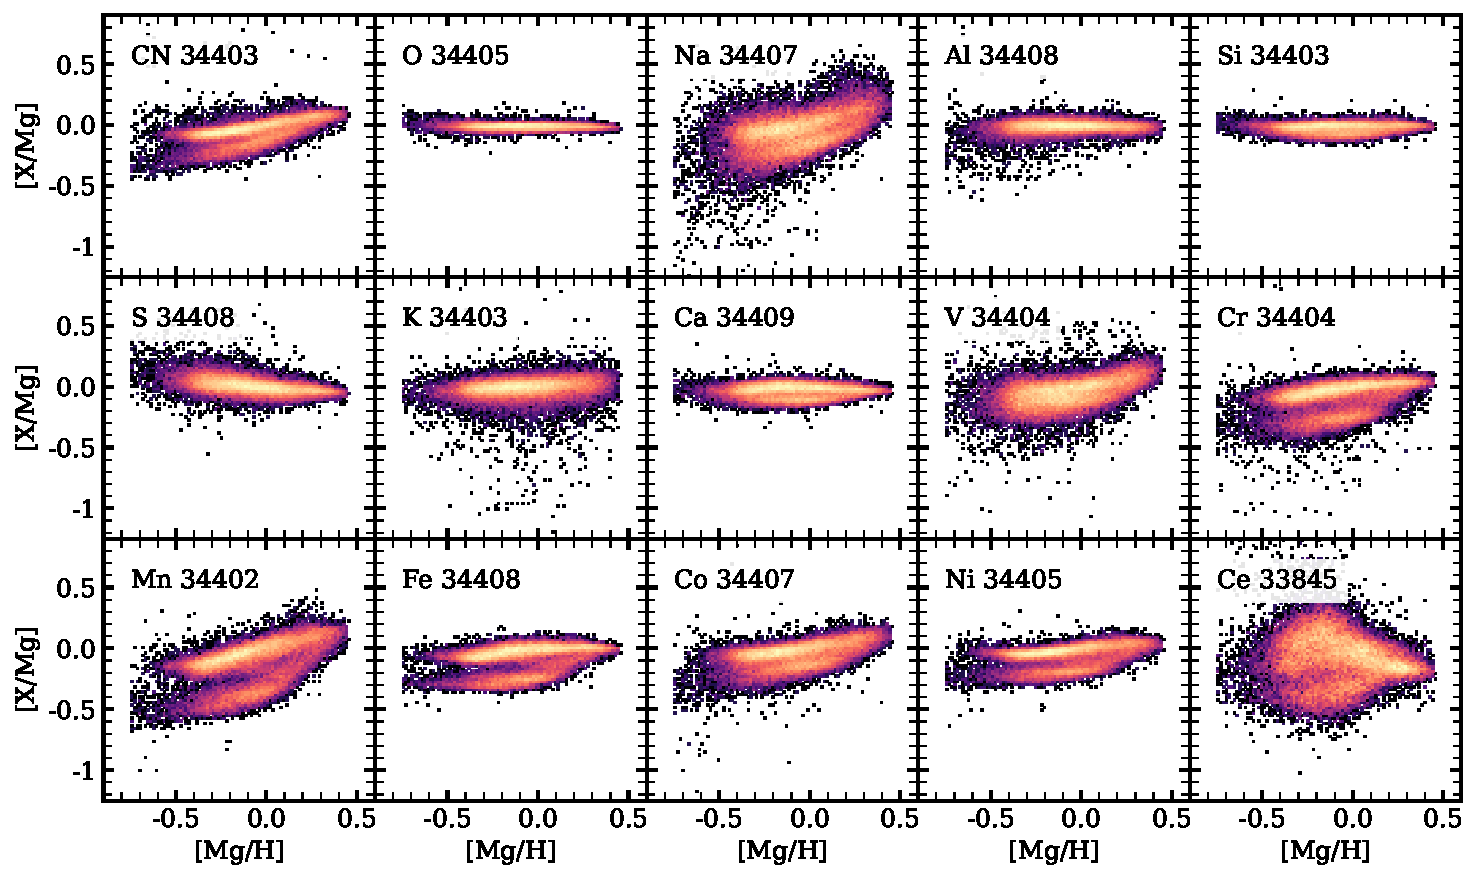
\includegraphics[width=\textwidth]{Figures/W22_xmg.pdf}
    \caption{Stellar abundance distributions for the W22 sample. The number in the top right corner indicates the number of stars used in the analysis of that element. Elements are ordered by atomic number.}
    \label{fig:w22_xmg}
\end{figure*}

\subsection{Expanded Sample}

While the W22 sample presented above is a good first test case of \name, we are interested in the behavior of our model when applied to a wider sample of data, in particular extending the metalicity range to lower values of [Mg/H]. To construct this sample, we apply the same quality cuts as taken by W22 (\texttt{STAR\_BAD} = 0, \texttt{NO\_ASPCAP\_RESULT} = 0, \texttt{FE\_H\_FLAG} = 0, \texttt{MG\_FE\_FLAG} = 0, and \texttt{EXTRATARG} = 0). We add a cut for stars with the \texttt{ROTATION\_WARNING} flag set. We additionally take the following sample selection cuts: 
\itemsep0em
\begin{itemize}
    \item S/N $\geq 100$
    \item $\logg =  0 - 2.5$ dex
    \item $\teff = 4000-4600$ K
    \item H $< 12$
\end{itemize}
We make no cuts on the [Mg/H] abundances. The wider $\logg$ range expands the sample of giants, though we select stars in the same small $\teff$ range as W22 to exclude the red clump \citep{vincenzo2021a} and cool stars that show abundance artifacts \citep{jonsson2020}. The $H$-band magnitude cut acts as a proxy for a distance cut \ejg{Add how many stars it excludes.}
Our final sample includes 51,386 stars and extends to [Mg/H]=-2.2. As in W22, we only analyze [X/Mg] abundances for stars where the [X/Fe] value is unflagged. This has a minimal effect for most elements but reduces the sample size to 49,851 for Ce. 

\begin{figure*}[htb!]
    \centering
    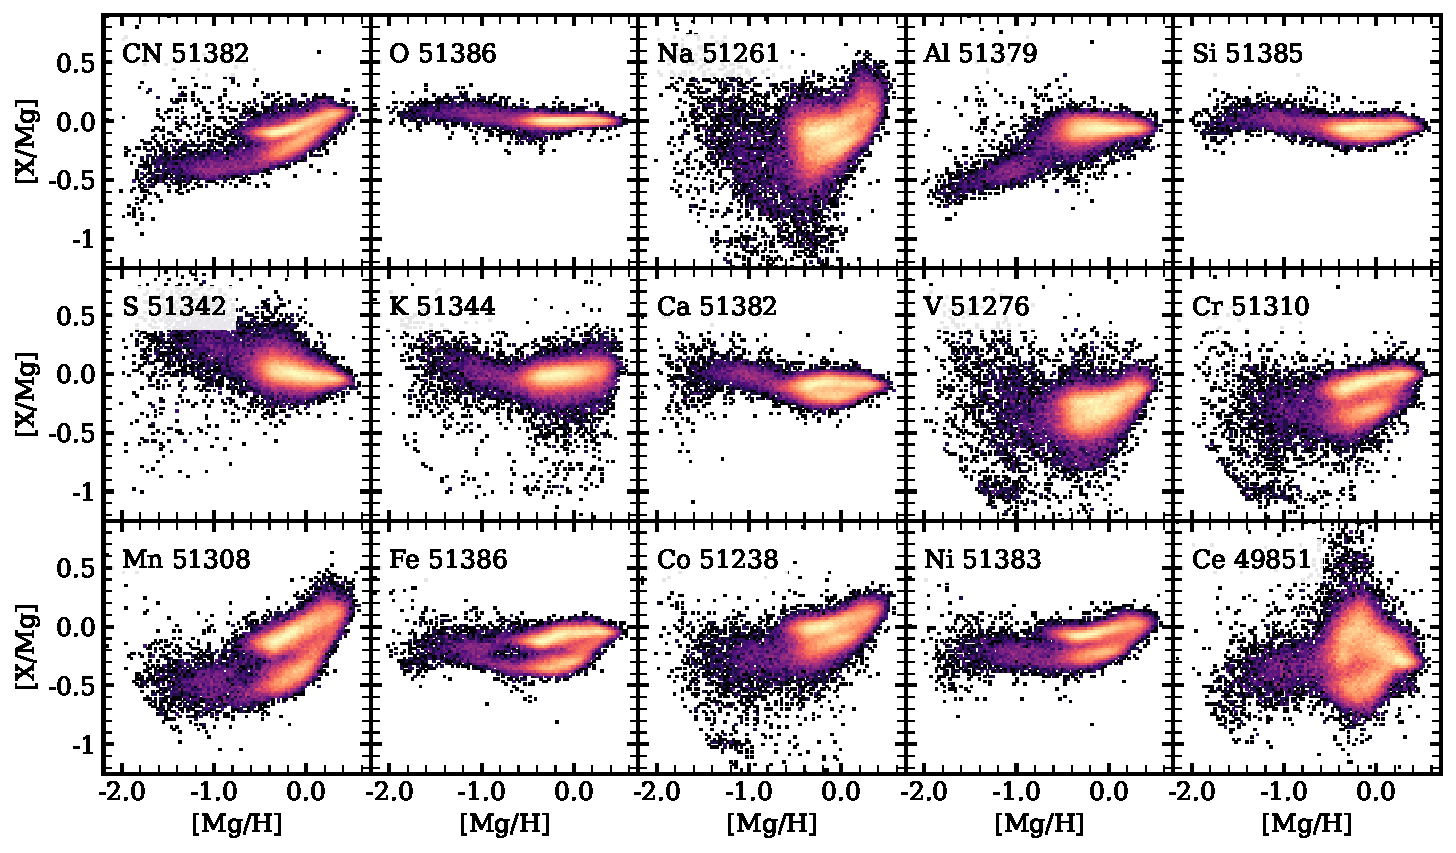
\includegraphics[width=\textwidth]{Figures/xmg.pdf}
    \caption{Stellar abundance distributions for our expanded stellar sample. The number in the top right corner indicates the number of stars used in the analysis of that element. Elements are ordered by atomic number. No zero-point offsets have been applied.}
    \label{fig:exp_xmg}
\end{figure*}

We plot the distribution of abundances in [X/Mg] vs. [Mg/H] for the expanded sample in Figure~\ref{fig:exp_xmg}. We do not apply zero-point offsets or temperature calibrations, as done in the W22 sample. 

The expansion of the data sample does introduce abundance systematics that the W22 cuts sought to exclude. As discussed in \citet{jonsson2020} and \citet{griffith2021a}, APGOEE DR16 and DR17 suffer from poorly understood abundance artifacts, such as a ``finger'' in [$\alpha$/M] and low-[X/Fe] banding in elements such as Al and Ni. In our expanded data set, we observe potential abundance artifacts in Al, K, V, and Cr, though the strict temperature cuts help to minimize these effects.  

\section{The K-Proccess Model}\label{sec:model}

As in W22 and G22, we propose that all stellar abundances can be described by the sum of $K$ nucleosynthetic process vectors and amplitudes. Each element has unique, metallicity-dependent process vectors that are universal for the stellar sample, while each star has unique process amplitudes. To begin, we consider the case for $K=2$ with a CCSN and SNIa process---the nucleosynthetic sources that dominate the production of the APOGEE elements \citep[e.g.,][]{andrews2017} such that

\begin{equation} \label{eq:m_ij}
    m_{ij} = \log_{10}(A_i^{\rm CC} \vec{q}_{{\rm CC}, j}^{\,Z} + A_i^{\rm Ia} \vec{q}_{{\rm Ia}, j}^{\,Z}) 
\end{equation}

where there are $i$ stars and $j$ elements described by process amplitudes $A_i^{\rm CC}$ and $A_i^{\rm Ia}$ and process vectors $\vec{q}_{{\rm CC}, j}^{\,Z}$ and $\vec{q}_{{\rm Ia}, j}^{\,Z}$. The observed value of $\xh$ can be described as the model plus observational noise and/or contributions from an additional non-CCSN nor SNIa processes:

\begin{equation} \label{eq:xh}
    \xh_{ij} = m_{ij} + \text{noise}.
\end{equation}

While such a model could be fit to a set stellar abundances, there are many degenerate solutions when there are no constraints on the model parameters. To better define our model and to collapse such degeneracies, we put forth a set a set of assumptions in the following section.

\subsection{Assumptions}\label{subsec:assumptions}

In the K-Process model, \name{}, we make the following assumptions:

\paragraph{1. Two processes}
The majority of $\alpha$, light odd-Z, and Fe-peak elements are dominantly produced by two sources: CCSN and SNIa. This is substantiated by theoretical yields \citep[e.g.,][]{anderson2019, rybizki2017} and past successful models (e.g., G22, \citealp{ting2022}, W22).
However, the assumption fails to allow for enrichment from other known sources, such as merging neutron stars, unique classes of supernoave, and AGB stars, the latter of which significantly contribute to C+N and Ce production.

\paragraph{2. Linearity}
At every metallicity, the abundances of a star can be expressed as a linear combination of two processes.
These processes themselves might depend on metallicity, but a linear sum is sufficient to explain all element abundances.
Because of dependences of yields on detailed abundances, and because different stars can get to their metallicities by different histories, this assumption must be slightly wrong in detail.

\paragraph{3. Non-negativity}
All process amplitudes for all elements are non-negative (elements considered here are only produced, not ever destroyed, by the two processes),
and all stars are made of a sum of the two non-negative processes.
This makes the model similar to a non-negative matrix factorization (\citealt{nnmf} \ejg{CITATION}). This assumption is not enforced in G22 and W22.

\paragraph{4. Mg is a pure CCSN}
All magnesium is produced in the CCSN process and none in the SNIa process. This is substantiated by theoretical yields \citep[e.g.,][]{anderson2019, rybizki2017}.
This breaks a rotational symmetry in the process space and makes the processes interpretable in terms of SN types.

\paragraph{5. Metallicity dependence}
The fact that all Mg is produced in the CCSN process is an assumption that is independent of metallicity.
All other process vectors are permitted to float as a function of metallicity.
The only exceptions are the Mg level in the CCSN process and the Fe level in the SNIa process, but these constraints are just model normalizations; they don't restrict the overall model freedom, which is about abundance ratios. \ejg{Check that this is right. Especially for Fe.}

\bigskip
The above assumptions  mirror the assumptions of prior work (G22, W22) but are weaker.
In particular, they don't assume anything about the relationships between the processes and the morphologies of observed element-abundance ratio diagrams.
In addition to the above assumptions, which are about nucleosynthesis, there are assumptions about the data:

\paragraph{6. APOGEE abundances and uncertainties}
We assume that the APOGEE abundances and uncertainties can be used for this project.
This is not the same as assuming that they are correct, but rather we are assuming that it is possible and useful to build an interpretable 2-process model to explain them. We describe the potential data systemtics in Section~\ref{sec:data}. The APOGEE errors are likely underestimated for many more challenging elements.

\paragraph{7. Likelihood function}
\ejg{Hogg to add}

\subsection{Model Constraints, Regularizations, and Implementation}\label{subsec:regularizations}

Some of the assumptions listed above directly translate to model constraints and regularization. Assumptions 1 and 2 form the basis of the model as described by Equation~\ref{eq:m_ij}. Assumption 3 is enforced by requiring that the process vectors and amplitudes are always greater than or equal to zero:
\begin{equation} \label{eq:constraint_zero}
    \vec{q}_{{\rm CC}, j}^{\,Z}, \, \vec{q}_{{\rm Ia}, j}^{\,Z} \geq 0 \quad \forall \; j
\text{   and   }
    A_i^{\rm CC}, \, A_i^{\rm Ia} \geq 0 \quad \forall \; i.
\end{equation}

To enforce assumptions 4 and 5, we initialize the model with specific values of $\vec{q}_{{\rm CC}}$ and $\vec{q}_{{\rm Ia}}$ and place regularizations ($\lambda$) on these constraints so that the model disfavors an alternative solution. In the initial model, we strongly require that
\begin{equation}\label{eq:qcc_solar}
    \vec{q}_{{\rm CC, Mg}}^{\,Z_{\odot}} = 1, \quad \vec{q}_{{\rm Ia, Mg}}^{\,Z_{\odot}} = 0, \quad 
    \vec{q}_{{\rm CC, Fe}}^{\,Z_{\odot}} = 0.5, \quad \vec{q}_{{\rm Ia, Fe}}^{\,Z_{\odot}} = 0.5
\end{equation}
at solar metallicity and 

\begin{equation}\label{eq:qcc_z}
    \vec{q}_{{\rm CC, Mg}}^{\,Z} = \vec{q}_{{\rm CC, Mg}}^{\,Z_{\odot}}, \quad 
    \vec{q}_{{\rm CC, Fe}}^{\,Z} = \vec{q}_{{\rm CC, Fe}}^{\,Z_{\odot}},  \quad 
    \vec{q}_{{\rm Ia, Fe}}^{\,Z} = \vec{q}_{{\rm Ia, Fe}}^{\,Z_{\odot}}
\end{equation}
at all other metallicities.
\ejg{Do we want to list regularization strengths? What is the difference between lambda a and lambda b in the notebook?} 
While the CCSN process constraint (that Mg is a pure CCSN element) is grounded in nucleosynthetic theory, there is no equivalent nucleosynthetic fact to constrain the SNIa process. We begin by initializing our model with the assumption that $\vec{q}_{{\rm CC, Fe}} = 0.5$, as in G22 and W22. This assumption places a pure CCSN star on the low metallicity [Mg/Fe] plateau near 0.3 dex, in agreement with APOGEE observations, but in contention with recent results from \citet{conroy2022} which places the [Mg/Fe] plateau near 0.6 dex. The flexibility of \name allows us to fit the model with different values of $\vec{q}_{{\rm CC, Fe}}$, allow for metallicity dependence in Fe CCSN and SNIa yields, and relax the regularization strengths in our initialization to see if the model prefers a different process vector. We explore different choices of $\vec{q}_{{\rm CC, Fe}}$ and regularization strengths in Section~\ref{subsec:fcc}.

We initialize the model according to Equations~\ref{eq:qcc_solar} and~\ref{eq:qcc_z}, setting all other $\vec{q}_{{\rm CC,}j}$ = $\vec{q}_{{\rm Ia,}j} = 0.5$ and all $A_i^{\rm CC} = A_j^{\rm Ia} = 0$. \ejg{Is this right?}

We then fit the $K$-process model to the W22 sample by minimizing the a chi-squared ($\chi^2$) with Gauss-Newton nonlinear least-squares solver in \texttt{jaxopt} where
\begin{equation}
    \chi^2 = \sum_{i=1}^{N} (\xh_{ij} - m_{ij})^{\rm T} c_j^{-1} (\xh_{ij} - m_{ij}) + \lambda~,
\end{equation}
and $c_j^{-1}$ is a matrix of the inverse variance squared,
\begin{equation}
    c^{-1} = \begin{bmatrix}
\frac{1}{\sigma_j^2} & 0 & ...\\
0 & \frac{1}{\sigma_j^2} & ... \\
0 & 0 & ... 
\end{bmatrix} .
\end{equation}
We fit the model to $N$ stars, such that $1 \leq i \leq N$, and $M$ elements, such that $1 \leq j \leq M$ where $j \in \{ \text{Mg, O, Si, S, Ca, CN, Na, Al, K, Cr, Fe, Ni, V, Mn, Co, Ce} \}$, by iteratively optimizing the process vectors (dubbed the q-step) and the process amplitudes (dubbed the A-step). \ejg{Add bit about how we determine how many times to repeat the iterations.}

\section{Optimization of \name} \label{sec:optimize}

\section{Comparing the W22 Two-Process Model and \name} \label{sec:results_W22}

\begin{itemize}
    \item Differences/similarities between the W22 fits and our fits. What do the differences mean
    \item Dependence of results on assumptions on assumptions such as the Fe yield/plateau value. Contrast the results for different assumptions and show the uncertainty in fcc 
\end{itemize}

\subsection{Dependence of $\fcc$ on Assumptions} \label{subsec:fcc}

\section{Application to a Broader Data Sample} \label{sec:results_broad}

\begin{itemize}
    \item Look at residuals from the K=2 fit, are there elements with correlated residuals? Are they the same as in W22? 
    \item show results for adding 3rd and 4th process to the data
\end{itemize}


\section{Summary}\label{sec:summary}

Notes

\begin{itemize}
    \item What is the connection between this model and latent variable models of machine learning
    \item Casual inferences - which abundances are caused by the Mg abundance and which are not (statistician perspective)
    \item Implications of differences at high metallicity
    \item Observational motivation for additional processes, what elements are critical for spectral surveys to observe
    \item Why this version of the 2 process model is more flexible than W22
\end{itemize}

\section{Acknowledgements}
It is a pleasure to thank
  Soledad Villar (JHU)
for valuable discussions.
This project benefited enormously from the Python package \texttt{jax} \citep{jax}.
E.J.G. is supported by an NSF Astronomy and Astrophysics Postdoctoral Fellowship under award AST-2202135.
CU Boulder Research Computing services and staff

% \software{Matplotlib \citep{hunter2007}, NumPy \citep{harris2020}, Pandas \citep{pandasa, pandasb}, Astropy \citep{astropy2013, astropy2018, astropy2022}, astroNN \citep{bovy2017}, EXOFASTv2 \citep{eastman2013, eastman2019}, iSpec \citep{blanco2014, blanco2019}, MOOG \citep{sneden1973}, galpy \citep{bovy2015, mackereth2018}}, jax \citep{jax}

\bibliography{sample631}{}
\bibliographystyle{aasjournal}

\end{document}

